\chapter{Eksperimentalna evalvacija}
Celostna evalvacija implementirane rešitve bi lahko zajemala več različnih vidikov, med drugim preverjanje izpolnjevanja vseh funkcijskih zahtev, določenih v fazi načrtovanja, ocenjevanje uporabniškega vmesnika in uporabniške izkušnje s pomočjo uporabniške študije ter analizo učinkovitosti izvedbe aplikacije, kot so odzivnost sistema, čas izvajanja simulacij in poraba sistemskih virov.

Ker takšna celovita evalvacija presega obseg diplomskega dela, se to delo osredotoča na eksperimentalno evalvacijo natančnosti razvite aplikacije. Natančnost simulacij predstavlja temeljno lastnost orodja za radijsko

Z eksperimentalno evalvacijo je bila preverjena natančnost razvite aplikacije ter temeljnega propagacijskega sistema SPLAT!, ki se uporablja za simulacijo radijskega širjenja. Evalvacija je bila izvedena na podlagi dejanskih terenskih meritev v realnem okolju, pri čemer je bila uporabljena obstoječa infrastruktura omrežja Meshtastic. Takšen pristop je omogočil izvajanje ponovljivih in nadzorovanih meritev v realnih pogojih delovanja sistema.

\paragraph{Meshtastic}
Meshtastic~\cite{meshtasticFirmware} je odprtokodna platforma za vzpostavljanje nizkoenergijskih brezžičnih omrežij na osnovi tehnologije LoRa, ki omogoča decentralizirano komunikacijo med večjim številom vozlišč v mrežnem tipu omrežja (angl. \emph{mesh network}). Vsako vozlišče lahko deluje kot oddajnik, sprejemnik in posrednik sporočil, kar omogoča razširjanje dosega omrežja brez potrebe po centralni infrastrukturi. Sistem omogoča dostop večjemu številu odjemalcev ter izmenjavo telemetrijskih in lokacijskih podatkov, hkrati pa
podpira integracijo z zunanjimi sistemi, na primer prek protokola MQTT, kar omogoča centralizirano zbiranje in analizo podatkov iz omrežja.

\section{Strojna in programska oprema}
Meritve so bile izvedene z uporabo odprtokodne programske opreme Meshtastic~\cite{meshtasticFirmware}, ki omogoča pošiljanje lokacijskih paketov ter njihovo posredovanje prek protokola MQTT. Sprejeti podatki so se samodejno shranjevali v podatkovno bazo skupaj s pripadajočimi metapodatki, kot so čas prejema, identifikacija oddajnika in sprejemnika ter izmerjena jakost signala (RSSI).

Uporabljena strojna oprema temelji na cenovno dostopnih mikrokontrolerjih ESP32 in nRF52 z vgrajeno podporo za komunikacijo LoRa. V eksperimentalnem okolju so bila uporabljena naslednja vozlišča:

\begin{itemize}
    \item Statično vozlišče \texttt{!7369fb6a}, ki temelji na platformi \href{https://store.rakwireless.com/products/wisblock-meshtastic-starter-kit}{\texttt{RAK Wireless RAK4631}}, opremljeni z anteno \href{https://www.alfa.com.tw/products/aoa-868-5acm?variant=36473962922056}{\texttt{Alfa 868~MHz 5~dBi}}.
    \item Statično vozlišče \texttt{!75f19024}, ki temelji na platformi \href{https://lilygo.cc/products/t3s3-v1-0}{\texttt{LilyGo T3 S3}}, opremljeni z anteno \href{https://mikrotik.com/product/868_omni_antenna}{\texttt{MikroTik 868~MHz 6.5~dBi}}.
    \item Mobilno vozlišče \texttt{!42e27414}, ki temelji na platformi \href{https://lilygo.cc/products/t-echo-lilygo}{\texttt{LilyGo T-Echo}}, opremljeni z anteno \href{https://www.alfa.com.tw/products/aoa-868-5acm?variant=36473962922056}{\texttt{Alfa 868~MHz 5~dBi}}.
\end{itemize}

Vsa oprema deluje na ISM frekvenčnem območju 868~MHz, z močjo 27~dBm. Lokacijski paketi so bili oddajani vsakih 15~s. Povprečna hitrost vožnje je znašala 50~km/h.

Pri izvajanju simulacij je bil uporabljen propagacijski model Irregular Terrain Model (ITM). Model je bil konfiguriran z uporabo parametrov delež lokacijskih situacij (angl. \emph{situation fraction}) in delež časa (angl. \emph{time fraction}), pri čemer sta bila oba nastavljena na vrednost 95. Takšna nastavitev pomeni, da model napoveduje radijske razmere, ki so izpolnjene v 95~\% prostorskih situacij in v 95~\% časa, kar predstavlja konzervativen pristop k ocenjevanju radijske pokritosti.

\section{Metodika meritev}

Merilno okolje je bilo sestavljeno iz dveh statičnih vozlišč in enega mobilnega vozlišča:
\begin{itemize}
    \item stacionarno vozlišče z anteno, nameščeno na stanovanjski hiši,
    \item solarno napajano stacionarno vozlišče, nameščeno na lokaciji Sv. Katarina,
    \item mobilno vozlišče, nameščeno na vozilu, ki je delovalo kot oddajnik.
\end{itemize}

\begin{figure}[H]
\centering
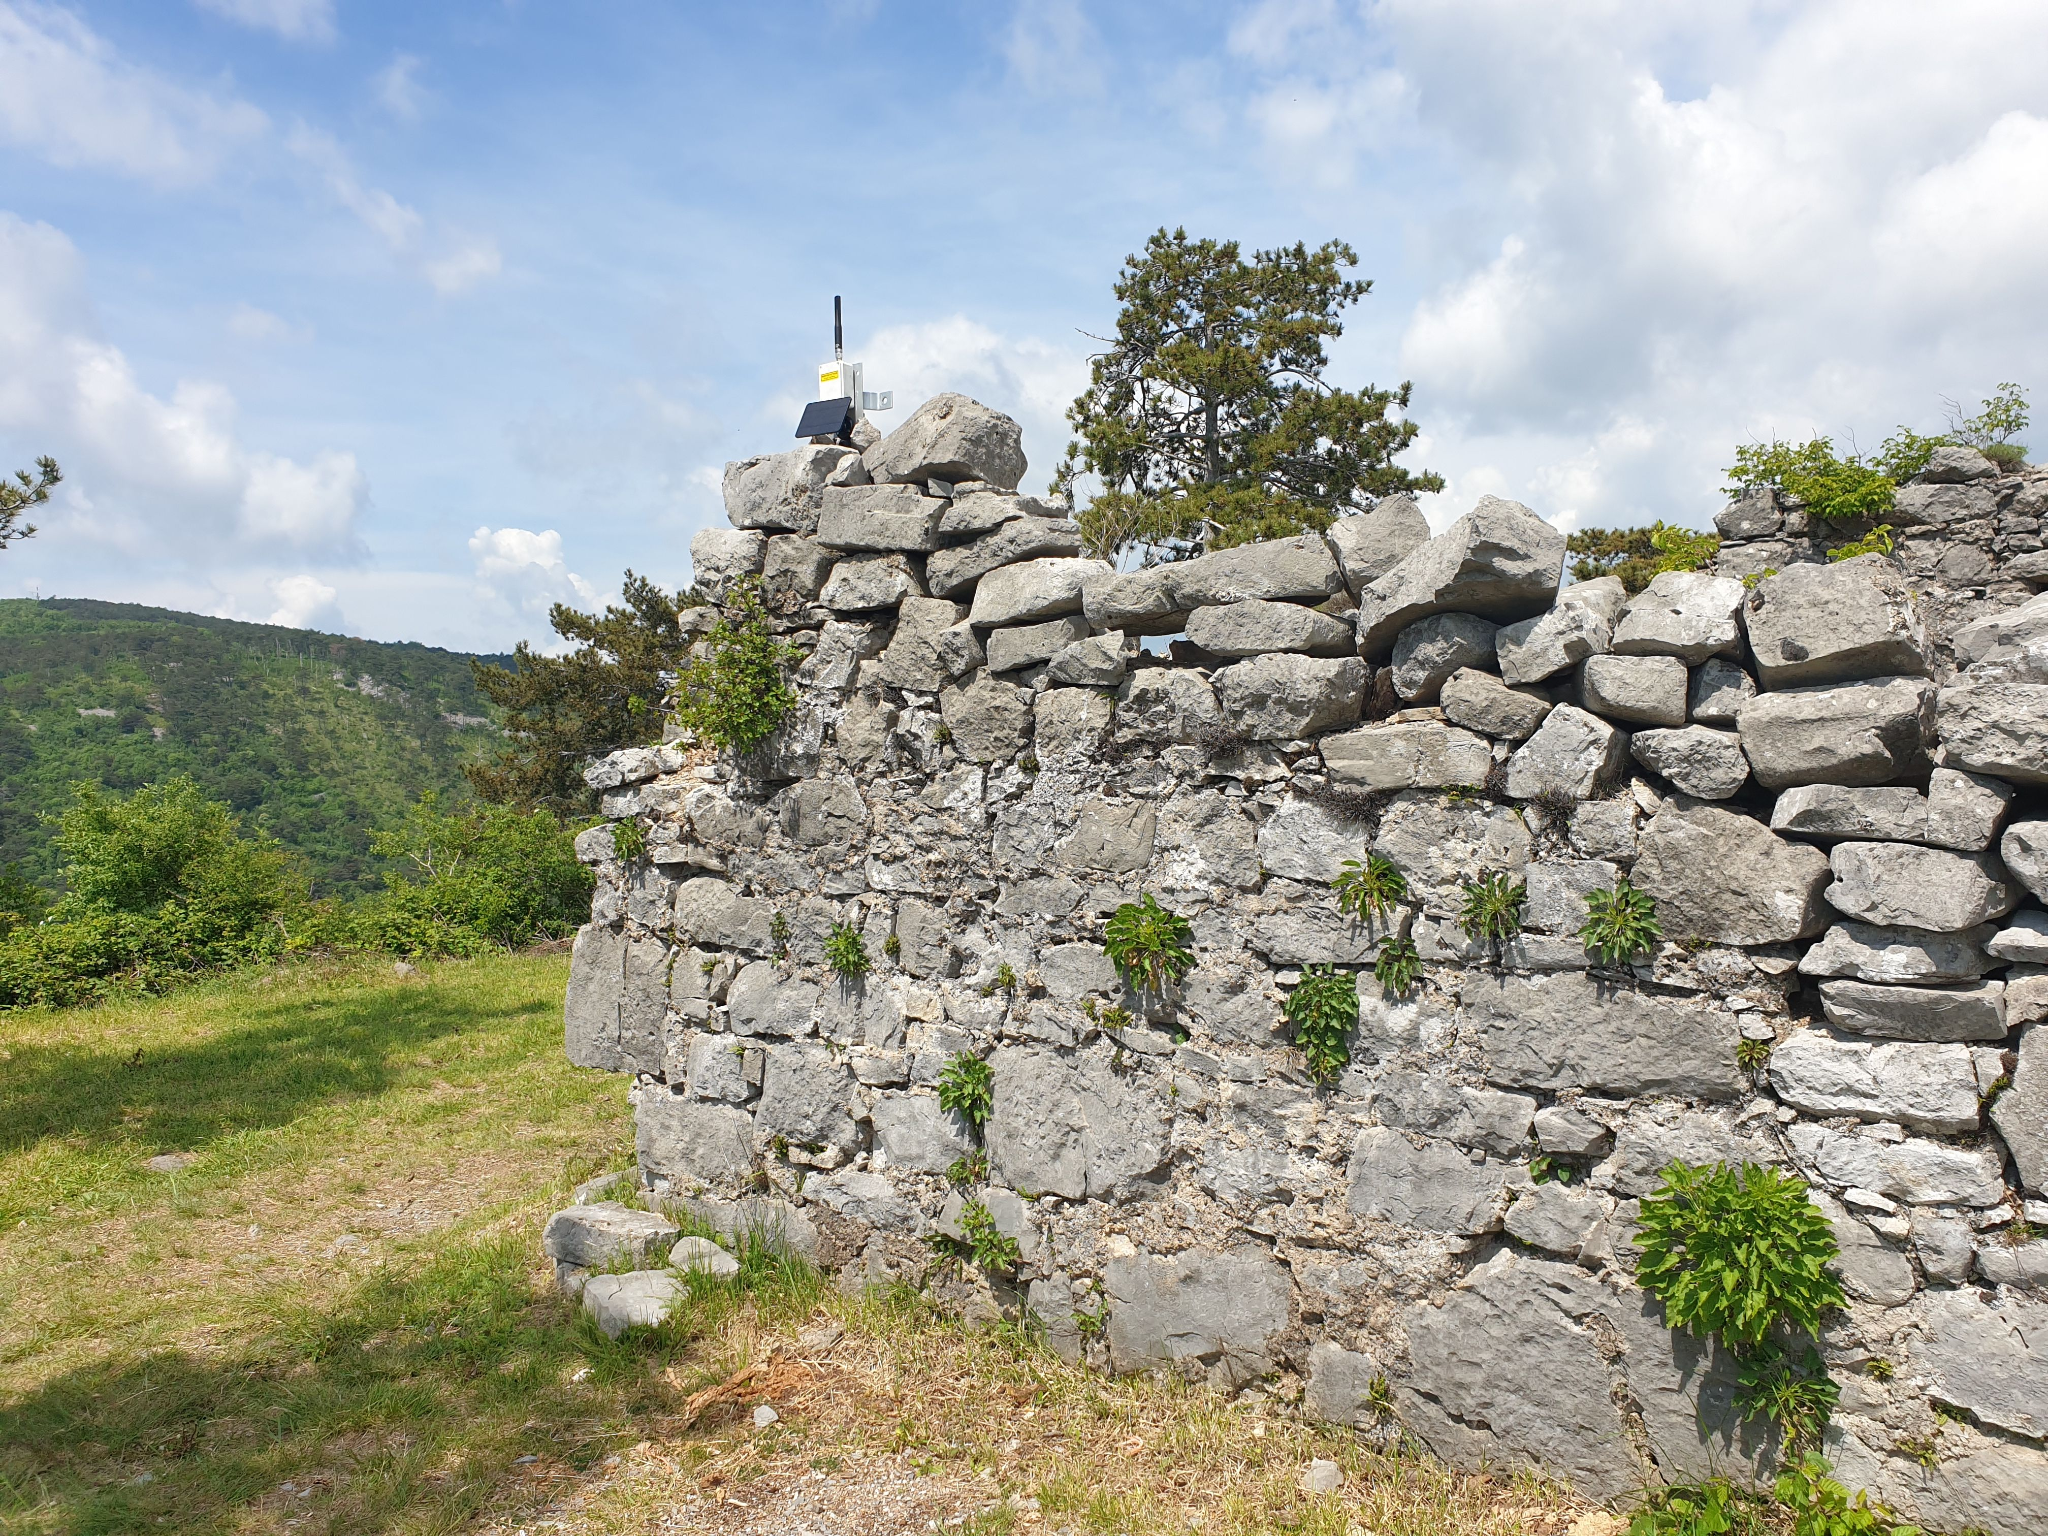
\includegraphics[width=\textwidth]{fotografije/sv-katarina-staticno-vozlisce.png}
\caption{Statično vozlišče na Sv. Katarini, !7369fb6a, 517~m nadmorske višine.}
\label{fig:sv-katarina-staticno-vozlisce}
\end{figure}

\begin{figure}[H]
\centering
\includegraphics[width=\textwidth]{fotografije/eksperimentalna-evalvacija-zemljevid-poti.jpg}
\caption{Zemljevid lokacij oddajanja in lokacij sprejemnikov}
\label{fig:eksperimentalna-evalvacija-zemljevid}
\end{figure}

Med meritvami se je vozilo, na katerem je bilo nameščeno mobilno vozlišče, premikalo po izbranem geografskem območju. Mobilno vozlišče je periodično oddajalo lokacijske pakete, pri čemer je bil časovni razmik med zaporednimi oddajami nastavljen na najmanj 15 sekund. S tem je bila zagotovljena skladnost z omejitvami radijskega spektra ter zmanjšana možnost preobremenitve omrežja. Višina oddajne antene na vozilu je bila približno 2 metra nad tlemi.

\begin{figure}[H]
\centering
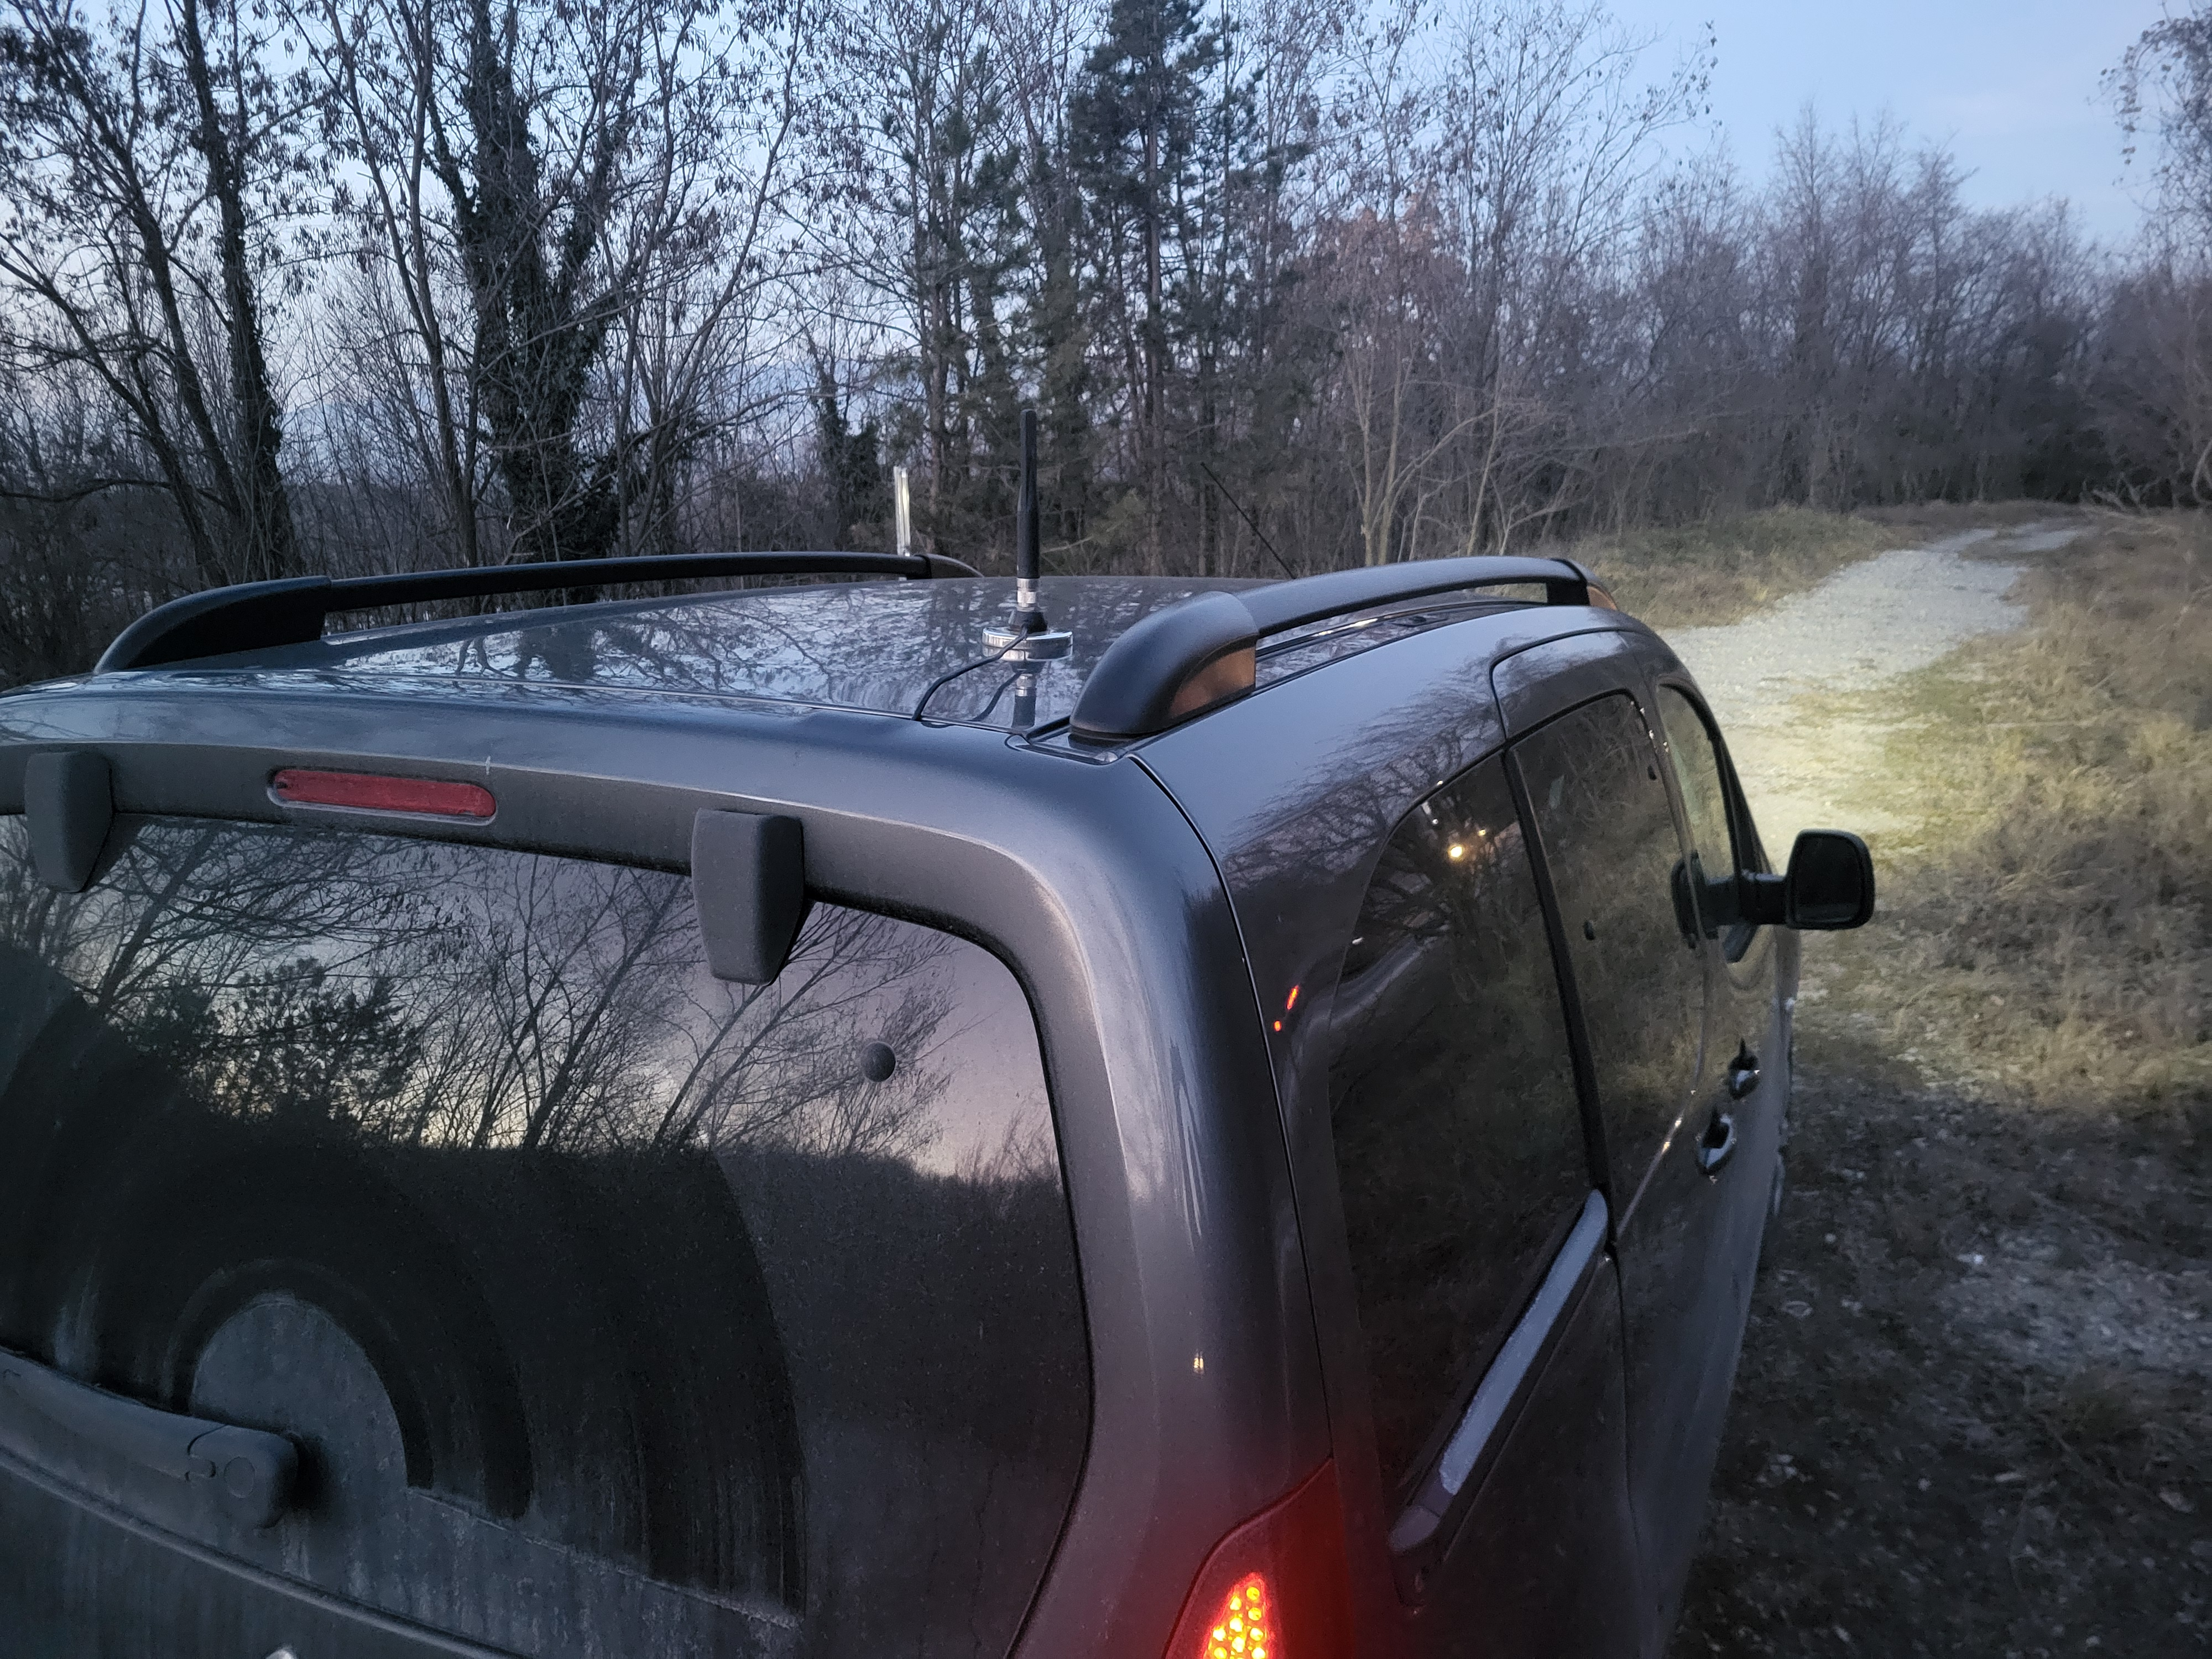
\includegraphics[width=1\textwidth]{fotografije/mobilni-node-avtomobil.jpg}
\caption{Osebni avtomobil, uporabljen kot mobilno vozlišče !42e27414.}
\label{fig:mobile-node-car}
\end{figure}

Statični vozlišči sta bili konfigurirani tako, da sta vse sprejete pakete posredovali prek protokola MQTT na osrednji strežnik. Na strežniku so se podatki samodejno shranjevali v podatkovno bazo skupaj z metapodatki, ki vključujejo čas prejema, identifikacijo oddajnika in sprejemnika ter izmerjeno jakost signala (RSSI).

Na ta način je bila vzpostavljena celovita zbirka merilnih podatkov, ki je omogočila analizo dosega, stabilnosti povezave ter prostorske porazdelitve jakosti signala. Zbrane meritve so bile v nadaljevanju uporabljene za primerjavo z rezultati simulacij in za ovrednotenje natančnosti uporabljenega radijskega modela.


\section{Rezultati}
Sprejemnik \texttt{!7369fb6a} je v času meritev skupno sprejel 434 paketov, medtem ko je nižje ležeči sprejemnik \texttt{!75f19024} sprejel 363 paketov. Razlika v številu sprejetih paketov je posledica različne višine namestitve anten in posledično drugačnih propagacijskih pogojev.

Sliki~\ref{fig:7369fb6a-val} in~\ref{fig:75f19024-val} prikazujeta primerjavo izmerjenih in simuliranih vrednosti RSSI za oba sprejemnika. Opaziti je, da simulacija v splošnem pravilno sledi trendu sprememb jakosti signala glede na položaj mobilnega vozlišča, vendar v določenih odsekih izrazito podcenjuje ali precenjuje dejansko izmerjene vrednosti.

\begin{figure}[H]
\centering
\includegraphics[width=1\textwidth]{fotografije/!7369fb6a_val.png}
\caption{Graf sprejemnika \texttt{!7369fb6a}, ki prikazuje meritev in simulacijo}
\label{fig:7369fb6a-val}
\end{figure}

\begin{figure}[H]
\centering
\includegraphics[width=1\textwidth]{fotografije/!75f19024_val.png}
\caption{Graf sprejemnika \texttt{!75f19024}, ki prikazuje meritev in simulacijo}
\label{fig:75f19024-val}
\end{figure}

Razlika med izmerjeno in simulirano jakostjo signala je bila definirana kot
\[
\Delta RSSI = RSSI_{\text{meritev}} - RSSI_{\text{simulacija}},
\]
kjer negativna vrednost pomeni, da je simulacija podcenila dejansko izmerjeno jakost signala, pozitivna vrednost pa pomeni njeno precenjevanje.

Z namenom podrobnejše analize so bili podatki razdeljeni v pet kategorij glede na geometrijske in propagacijske pogoje med oddajnikom in sprejemnikom:

\begin{itemize}
    \item \textbf{Vsi paketi} – združena napaka vseh prejetih paketov, ne glede na propagacijske pogoje.
    \item \textbf{LOS} – napake paketov v primerih, ko sta imela oddajnik in sprejemnik med seboj vidno linijo (angl. \emph{line of sight}).
    \item \textbf{NLOS} – napake paketov v primerih, ko med oddajnikom in sprejemnikom ni bilo vidne linije.
    \item \textbf{NF60} – napake paketov v primerih, ko je bila prva Fresnelova cona prekrita približno do 60~\%.
    \item \textbf{NFF} – napake paketov v primerih, ko je bila prva Fresnelova cona v celoti prekrita.
\end{itemize}

Na obeh grafih~\ref{fig:7369fb6a-diff-box} in~\ref{fig:75f19024-diff-box} lahko vidimo, da je simulacija NLOS povezave močno podcenila. Ostale vrste povezav pa se gibljejo na precenjenem območju. 

\begin{figure}[H]
\centering
\includegraphics[width=1\textwidth]{fotografije/!7369fb6a_diff.png}
\caption{Graf sprejemnika \texttt{!7369fb6a}, ki prikazuje napako med meritvijo in simulacijo, glede na vidnost.}
\label{fig:7369fb6a-diff}
\end{figure}

\begin{figure}[H]
\centering
\includegraphics[width=1\textwidth]{fotografije/!75f19024_diff.png}
\caption{Graf sprejemnika \texttt{!75f19024}, ki prikazuje napako med meritvijo in simulacijo, glede na vidnost.}
\label{fig:75f19024-diff}
\end{figure}

Porazdelitev napak po posameznih kategorijah je prikazana na slikah~\ref{fig:7369fb6a-diff-box} in~\ref{fig:75f19024-diff-box}. Škatle z brki jasno pokažejo, da je razpršenost napak močno odvisna od vidnosti in stopnje oviranosti Fresnelove cone.

\begin{figure}[H]
\centering
\includegraphics[width=1\textwidth]{fotografije/!7369fb6a_diff_box.png}
\caption{Graf sprejemnika \texttt{!7369fb6a}, ki prikazuje napako med meritvijo in simulacijo, glede na vidnost.}
\label{fig:7369fb6a-diff-box}
\end{figure}

\begin{figure}[H]
\centering
\includegraphics[width=1\textwidth]{fotografije/!75f19024_diff_box.png}
\caption{Graf sprejemnika \texttt{!75f19024}, ki prikazuje napako med meritvijo in simulacijo, glede na vidnost.}
\label{fig:75f19024-diff-box}
\end{figure}


Sliki~\ref{fig:7369fb6a-diff-vs-length} in~\ref{fig:75f19024-diff-vs-length} prikazujeta tudi odvisnost napake simulacije $\Delta RSSI$ od dolžine povezave. Vsaka točka predstavlja razliko med izmerjeno in simulirano vrednostjo RSSI pri določeni razdalji med oddajnikom in sprejemnikom.

Pri sprejemniku \texttt{!7369fb6a} je opazna izrazita negativna korelacija med dolžino povezave in napako simulacije, kar potrjuje tudi linearni regresijski model z razmeroma visokim koeficientom determinacije ($R^2 = 0.428$). To pomeni, da simulacija z naraščajočo razdaljo vse pogosteje podcenjuje dejansko izmerjeno jakost signala.

Pri sprejemniku \texttt{!75f19024} z nižjo nadmorsko višino je korelacija med razdaljo in napako bistveno šibkejša ($R^2 = 0.061$), kar kaže na večji vpliv lokalnih dejavnikov, kot so višina antene, ovire in topografija. Kljub temu je tudi v tem primeru opazen splošen trend naraščanja absolutne napake z razdaljo.

Rezultati potrjujejo, da natančnost simulacij z uporabo determinističnega propagacijskega modela upada z naraščajočo dolžino povezave, zlasti v primerih brez vidne linije, kjer imajo lokalni propagacijski pojavi bistveno večji vpliv kot sama razdalja.


\begin{figure}[H]
\centering
\includegraphics[width=\textwidth]{fotografije/!7369fb6a_diff_vs_length_non_los.png}
\caption{Odvisnost napake simulacije od dolžine povezave za sprejemnik \texttt{!7369fb6a}}
\label{fig:7369fb6a-diff-vs-length}
\end{figure}

\begin{figure}[H]
\centering
\includegraphics[width=\textwidth]{fotografije/!75f19024_diff_vs_length_non_los.png}
\caption{Odvisnost napake simulacije od dolžine povezave za sprejemnik \texttt{!75f19024}}
\label{fig:75f19024-diff-vs-length}
\end{figure}


\section{Kalibracija na podlagi meritev}

Na podlagi rezultatov eksperimentalne evalvacije je bilo ugotovljeno, da se v primerih brez vidne linije (NLOS) napaka simulacije sistematično spreminja z razdaljo med oddajnikom in sprejemnikom. Opazna je bila odvisnost med dolžino povezave in razliko med izmerjeno ter simulirano vrednostjo RSSI, kar kaže na prisotnost razdaljsko odvisnega sistematičnega odklona v uporabljenem propagacijskem modelu.

Z namenom izboljšanja natančnosti napovedi je bila izvedena kalibracija simulacijskih rezultatov na podlagi dejanskih meritev. Kalibracija je temeljila na linearni regresiji, s katero je bila modelirana odvisnost napake simulacije od razdalje. Izračunani linearni regresijski model je bil nato uporabljen za korekcijo simuliranih vrednosti RSSI.

Za preprečevanje pristranskosti in preverjanje posplošljivosti kalibracije so bili razpoložljivi podatki razdeljeni na dva disjunktna dela. Prva polovica meritev je bila uporabljena za izračun regresijskega modela, druga polovica pa za neodvisno evalvacijo učinkovitosti kalibracije. Meritve v obeh delih so bile izvedene na različnih odsekih poti, kar zagotavlja, da kalibracija ni prilagojena specifični trasi ali lokalnim značilnostim okolja.

Na sliki~\ref{fig:7369fb6a-box-before} je prikazana porazdelitev napak simulacije glede na propagacijske pogoje pred izvedeno kalibracijo, medtem ko slika~\ref{fig:7369fb6a-box-after} prikazuje porazdelitev napak po uporabi kalibracijskega modela.

\begin{figure}[H]
\centering
\includegraphics[width=\textwidth]{fotografije/!7369fb6a_diff_box_2_half.png}
\caption{Porazdelitev napake simulacije glede na propagacijske pogoje pred kalibracijo za sprejemnik \texttt{!7369fb6a}}
\label{fig:7369fb6a-box-before}
\end{figure}

\begin{figure}[H]
\centering
\includegraphics[width=\textwidth]{fotografije/!7369fb6a_diff_box_2_half_optimized.png}
\caption{Porazdelitev napake simulacije glede na propagacijske pogoje po kalibraciji za sprejemnik \texttt{!7369fb6a}}
\label{fig:7369fb6a-box-after}
\end{figure}

Učinek kalibracije je bil ocenjen s primerjavo porazdelitve napak pred in po kalibraciji. Škatle z brki (box-plot) jasno pokažejo, da se je po kalibraciji mediana napak v NLOS pogojih približala vrednosti 0~dB, kar kaže na zmanjšanje sistematičnega odklona simulacijskih rezultatov.

Rezultati potrjujejo, da lahko preprosta linearna kalibracija na podlagi terenskih meritev izboljša ujemanje med simuliranimi in izmerjenimi vrednostmi RSSI, zlasti v NLOS pogojih, kjer osnovni propagacijski model deluje konzervativno.


\section{Razprava}

Rezultati eksperimentalne evalvacije kažejo jasno odvisnost natančnosti simulacij od propagacijskih pogojev. V primerih z vidno linijo (LOS) je razlika med izmerjenimi in simuliranimi vrednostmi RSSI relativno majhna, mediane napak pa se pri obeh sprejemnikih gibljejo okoli 10~dB. Takšna stopnja ujemanja potrjuje, da uporabljeni radijski model v pogojih vidne linije ustrezno opisuje osnovne propagacijske mehanizme, kar je skladno z ugotovitvami iz literature~\cite{6618611}.

V primerih brez vidne linije (NLOS) so odstopanja bistveno večja, pri čemer se mediane napak gibljejo okoli 20~dB. Simulacija v teh pogojih pogosto podcenjuje dejanski doseg povezave, kar se odraža v negativni sistematični napaki in izrazito večji razpršenosti podatkov. Posamezna odstopanja presegajo 40~dB, kar kaže na omejitve determinističnega propagacijskega modela pri opisovanju kompleksnih mehanizmov širjenja signala v razgibanem terenu.

Dodatna analiza je pokazala, da ima dolžina povezave vpliv na napako simulacije, zlasti v pogojih brez vidne linije. Z naraščajočo razdaljo med oddajnikom in sprejemnikom se sistematično povečuje absolutna napaka med izmerjenimi in simuliranimi vrednostmi RSSI, kar potrjuje negativna korelacija, ugotovljena z linearno regresijsko analizo.
